\documentclass{beamer}

\usepackage[utf8]{inputenc}
\usecolortheme{beaver}
\usepackage{caption}
\usepackage{subcaption}
\usepackage{mathtools}
\usepackage{todonotes}
\usepackage{amsmath}
\usepackage{bm}
\usepackage{listings}
\usepackage{ragged2e}
\usepackage{titlecaps}
\usepackage{fancyvrb}

\def\ci{\perp\!\!\!\!\!\perp}

\newtheorem{proposition}{Proposition}
\Addlcwords{for a is but and with of in as the etc on to if}

\setbeamertemplate{section in toc}{\inserttocsectionnumber.~\inserttocsection}
\usetheme{Boadilla}
\makeatletter
\setbeamertemplate{footline}{%
    \leavevmode%
    \hbox{%
        \begin{beamercolorbox}[wd=.3\paperwidth,ht=2.25ex,dp=1ex,center]{author in head/foot}%
            \usebeamerfont{author in head/foot}\insertshortauthor\expandafter\beamer@ifempty\expandafter{\beamer@shortinstitute}{}{~~(\insertshortinstitute)}
        \end{beamercolorbox}%
        \begin{beamercolorbox}[wd=.55\paperwidth,ht=2.25ex,dp=1ex,center]{title in head/foot}%
            \usebeamerfont{title in head/foot}\insertshorttitle
        \end{beamercolorbox}%
        \begin{beamercolorbox}[wd=.15\paperwidth,ht=2.25ex,dp=1ex,right]{date in head/foot}%
            \usebeamerfont{date in head/foot}\insertshortdate{}\hspace*{2em}
            \insertframenumber{} / \inserttotalframenumber\hspace*{2ex} 
        \end{beamercolorbox}}%
        \vskip0pt%
    }
\makeatother

\begin{document}

\title[]{Statistical and Causal Robustness for Causal Null Hypothesis Tests}
\date{}

\maketitle

\begin{frame}{Background}
	\begin{figure}
		\center
		\includegraphics[page=1]{figures.pdf}
		\caption*{Workflow for estimating causal effect from observational data}
	\end{figure}

	\vspace{1em}
	\begin{itemize}
		\item Difficult to construct DAG from data.
		\item Typically done by hand based on domain knowledge.
		\item Different structure learning algorithms are available.
		\item No easy way to test whether the DAG is correct.
	\end{itemize}	
\end{frame}

\begin{frame}{Background}
	\begin{figure}
		\center
		\includegraphics[page=2]{figures.pdf}
	\end{figure}
	\vspace{1em}
	\begin{itemize}
		\item Given a DAG, check whether parameter is estimable.
			\begin{figure}
				\center
				\begin{subfigure}{0.25 \textwidth}
					\center
					\includegraphics[page=4, scale=0.8]{figures.pdf}
				\end{subfigure}%
				\begin{subfigure}{0.25 \textwidth}
					\center
					\includegraphics[page=5, scale=0.8]{figures.pdf}
				\end{subfigure}
			\end{figure}
		\item do-calculus gives a complete solution but difficult to apply in practice.
		\item Special case solutions: Backdoor, Front-door, Instrumental Variables (IV).
		\item Each criterion makes different assumptions about the specified model.
		\item Assumptions are difficult to test in data.
	\end{itemize}
\end{frame}

\begin{frame}{Background}
	\begin{figure}
		\center
		\includegraphics[page=3]{figures.pdf}
	\end{figure}
	\vspace{1em}
	\begin{itemize}
		\item If the model is correctly specified, and identification criterion assumptions are satisfied, an estimator can be used.
		\item The estimator makes further assumptions about the data such as linearity, distribution, etc.
		\item Statistically robust estimators are available, i.e. unbiased, fast convergence, etc.
	\end{itemize}
\end{frame}

\begin{frame}{Problem Statement}
	\begin{itemize}
		\item Develop a statistical test to test whether a causal effect is present. 
			$$ H_0: \beta = 0 $$
		\item As specifing a single correct model is difficult, the test works on a set of models.
		\item The statistical test works if even one of the models is correct.
		% \item It is challenging to come up with a single correct specification of the model.
		% \item Instead, use a bunch of different model. And the paper proposes a robustness test on this set of models.
		% \item The test check if the causal assumption is true if atleast one of the specified model is correct.
		% \item They use something called Evidence Factors to combine the results from testing on the models.
		% \item Limited to semi-parameteric estimation methods. For convergence properties of the test??
	\end{itemize}
\end{frame}

\begin{frame}{Example}
	\begin{itemize}
		\item Test whether there is an effect of \textbf{smoking} on \textbf{glucose levels}.
		\item Given a dataset $ D = \{ C, Z, A, M, Y \} $.
			\begin{itemize}
				\item Treatment ($ A $): Smoking status.
				\item Outcome ($ Y $): Glucose level.
				\item Baseline covariates ($ C $): Age, sex, BMI, past history of heart disease, and past glucose level.
				\item Mediator ($ M $): Hypertension.
				\item IV ($ Z $): Past hypertension.
			\end{itemize}
		\item Estimate the average causal effect (ACE) of smoking on glucose.
	\end{itemize}
			$$ \beta = \mathbb{E}[Y(A=1)] - \mathbb{E}[Y(A=0)] $$
\end{frame}

\begin{frame}{Example}
	\begin{figure}
		\center
		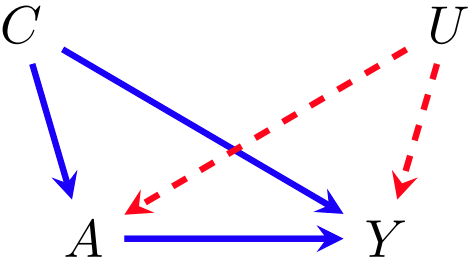
\includegraphics[scale=0.2]{m1.png}
	\end{figure}
	\begin{itemize}
		\item Backdoor model. Adjusting on $ C $ would give us the estimate for $ A \rightarrow Y $.
		\item But no unobserved confounding can be present $ U $, otherwise the effect is not identified.
		\item But possible that we missed to collect data on some of our covariates. For example, health consciousness is an unmeasured covariate. %TODO: Add what could be covariate.
	\end{itemize}
	$$ \Psi_{1, P} = \mathbb{E}[\mu(1, C) - \mu(0, C)] $$
	$$ \mu(a, c) = \mathbb{E}(Y | A=a, C=c) $$
\end{frame}

\begin{frame}{Example}
	\begin{figure}
		\center
		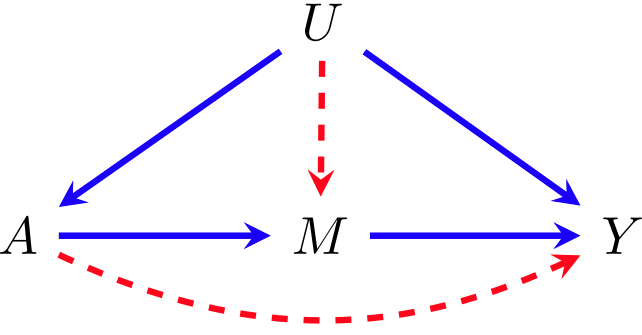
\includegraphics[scale=0.2]{m2.png}
	\end{figure}
	\begin{itemize}
		\item Front-door model. $ M $ is the mediator here.
		\item Model allows for unobserved confounding between the treatment and outcome.
		\item But there can't be an effect between the unobserved variable and the mediator or direct effect between the treatment and outcome.
	\end{itemize}
	$$ \Psi_{2, P} = \mathbb{E}[\mathbb{E}[\gamma(M, C) | A = 1, C] - \mathbb{E}[\gamma(M, C) | A =0, C]] $$
	$$ \gamma(m, c) = \mathbb{E}[\mu(m, A, c) | C=c]; \mu(m, a, c) = \mathbb{E}(Y | M=m, A=a, C=c) $$
\end{frame}

\begin{frame}{Example}
	\begin{figure}
		\center
		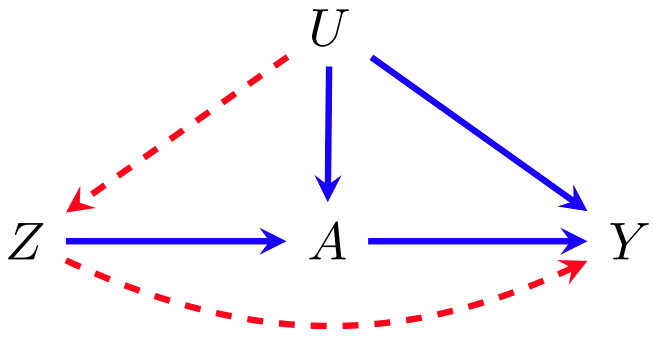
\includegraphics[scale=0.2]{m3.png}
	\end{figure}
	\begin{itemize}
		\item Instrumental Variable model. $ Z $ is the IV.
		\item $ Z $ should not be correlated with $ Y $ unless all information goes through $ A $.
	\end{itemize}
	$$ \Psi_{3, P} = \frac{\mathbb{E}(Y | Z = 1) - \mathbb{E}(Y | Z = 0)}{\mathbb{E}(A | Z = 1) - \mathbb{E}(A | Z=0)} $$
\end{frame}

\begin{frame}{Example}
	\begin{itemize}
		\item If a semi-parameteric estimator of the corresponding parameter exist, it can be used to construct a statistically robust hypothesis test of the causal null hypothesis $ \beta = 0 $.
		\item 
	\end{itemize}
\end{frame}

\begin{frame}{Evidence Factors}
\end{frame}

\begin{frame}{Proposed Solution Overview}
	$$ H_{0}: \beta = 0 $$
	IID data $ O_1, \cdots, O_n $ from unknown distribution $ P $.
	Considering $ K > 1 $ causal models $ M_1, \cdots, M_k $.
	$ \Psi_{k, P} $ is the identifying functional for $ \beta $ under $ M_k $.
\end{frame}

\begin{frame}{Proposed Solution}
\end{frame}

\begin{frame}{Applied to Practical Example}
\end{frame}

\begin{frame}{Real Data Example}
\end{frame}

\begin{frame}{Conclusion}
\end{frame}

\end{document}
